\documentclass[letterpaper, 12pt]{article}
\usepackage{amsmath}
\usepackage[margin=1in]{geometry}
\usepackage{adjustbox}
\usepackage{graphicx}
\usepackage[final]{pdfpages}
\usepackage{bm}
\usepackage{sectsty}
\usepackage{titlesec}
\usepackage{lipsum}
\usepackage{subcaption}
\usepackage{listings}
\usepackage{pgffor}
\usepackage{rotating}
\usepackage{xcolor}  
\usepackage{amsthm}
\usepackage{csvsimple}
\usepackage{enumitem}
\usepackage{amssymb} 
\usepackage{amsfonts}
\usepackage{tikz}
\usepackage{tikz-3dplot}
% \setlength{\tabcolsep}{0.5cm} 
\newcommand{\thickhat}[1]{\mathbf{\hat{\text{$#1$}}}}
\renewcommand{\lstlistingname}{Program}

\newtheoremstyle{custom}
  {3pt}
  {3pt}
  {\itshape}
  {} 
  {\bfseries}
  {. }  
  { }   
  {\thmname{#1} \thmnumber{#2} \thmnote{ #3}}

\theoremstyle{custom}


\newtheorem{definition}{Definition}
% \newtheorem{theorem}{Theorem}
\newtheorem*{theorem}{Theorem}
\sectionfont{\fontsize{12}{15}\selectfont}
\titleformat{\section}
{\normalfont\normalsize\bfseries}
{(\thesection)}{1em}{}

\title{Divergence and Curl}
\author{Masaru Sawata}
\begin{document}
\maketitle
There are several forms of the difinition of divergence and curl. One of them is using the integral form.
\begin{definition}[Divergence]
  The divergence of a vector field $\vec{v}$ is defined as
  \begin{equation*}
    \nabla \cdot \vec{v} = \lim_{V \rightarrow 0} \frac{\displaystyle \int_{\partial \Omega} \vec{v} \cdot \vec{dS}}{V}
  \end{equation*}
  where $\partial \Omega$ is the closed surface and the volume inside $\partial \Omega$ is $V$
\end{definition}

\bigskip

\begin{definition}[Curl]
  The curl of a vector field $\vec{v}$ is defined as
  \begin{equation*}
    \left( \nabla \times \vec{v} \right) \cdot \vec{n} = \lim_{S \rightarrow 0} \frac{\displaystyle \oint_{C} \vec{v} \cdot \vec{dr}}{S}
  \end{equation*}
  where $\vec{n}$ is a unit vector in an arbitrary direction, $S$ is an area of plane perpendicular to $\vec{n}$ and closed by curve $C$
\end{definition}

\bigskip

\begin{theorem}[Gauss Divergence Theorem]
  \begin{equation*}
    \int_{\Omega} \nabla \cdot \vec{v} dV = \int_{\partial \Omega} \vec{v} \cdot \vec{dS}
  \end{equation*}
\end{theorem}
\begin{proof}
  First, we divide the region $\Omega$ into $n$ regions. Each region is denoted as $\Omega_i (i=1,2,\cdots , n)$.
  We can write the RHS of the theorem as follows.
  \begin{equation*}
    \int_{\partial \Omega} \vec{v} \cdot \vec{dS} = \sum_{i=1}^{n}\int_{\partial \Omega_i} \vec{v} \cdot \vec{dS}
  \end{equation*}
  This is because the surface integral on the boundary between $\Omega_i$ and $\Omega_j$ cancels out due to the oposite direction of $\vec{dS}$.
  Let $V_i$ be the volume of the region $\Omega_i$. In addition, we define $| \Delta |=\max \{ V_i;1 \leq i \leq n \}$.
  We can increase the number of division so that $| \Delta |$ becomes less than any positive value. Therefore,
  \begin{align*}
    \int_{\partial \Omega} \vec{v} \cdot \vec{dS} 
    &= \sum_{i=1}^{n}\int_{\partial \Omega_i} \vec{v} \cdot \vec{dS}\\
    &= \sum_{i=1}^{n}\frac{\displaystyle \int_{\partial \Omega_i} \vec{v} \cdot \vec{dS}}{V_i} V_i\\
    &\rightarrow \int_{\Omega} \nabla \cdot \vec{v} dV \quad (|\Delta| \rightarrow 0)
  \end{align*}
\end{proof}

\bigskip

\begin{theorem}[Stokes' Theorem]
  \begin{equation*}
    \int_{\Gamma} \left( \nabla \times \vec{v} \right) \cdot \vec{ds} = \oint_{C} \vec{v} \cdot \vec{dr}
  \end{equation*}
\end{theorem}
\begin{proof}
  First, we divide the surface $\Gamma$ into $n$ surfaces. Each surface is denoted as $\Gamma_i (i=1,2,\cdots , n)$, 
  and the closed loop around $\Gamma_i$ is $C_i$
  We can write the RHS of the theorem as follows.
  \begin{equation*}
    \oint_{C} \vec{v} \cdot \vec{dr} = 
    \sum_{i=1}^{n} \oint_{C_i} \vec{v} \cdot \vec{dr}
  \end{equation*}
  This is because the integral on the boundary between $\Gamma_i$ and $\Gamma_j$ cancels out due to the opposite direction of the integral.
  Let $S_i$ be the are of the surface $\Gamma_i$. In addition, we define $| \Delta |=\max \{ S_i;1 \leq i \leq n \}$.
  We can increase the number of division so that $| \Delta |$ becomes less than any positive value. Therefore,
  \begin{align*}
    \oint_{C} \vec{v} \cdot \vec{dr} 
    &= \sum_{i=1}^{n} \oint_{C_i} \vec{v} \cdot \vec{dr}\\
    &= \sum_{i=1}^{n} \frac{\displaystyle \oint_{C_i} \vec{v} \cdot \vec{dr}}{S_i} S_i\\
    &\rightarrow \int_{\Gamma} \left( \nabla \times \vec{v} \right) \cdot \vec{dS} \quad (|\Delta| \rightarrow 0)
  \end{align*}
\end{proof}

\bigskip

We can derive the divergence in Cartesian coordinate by considering the rectangular prism shown in Figure \ref{fig: 1}.

\begin{figure}[htbp]
  
\begin{center}
  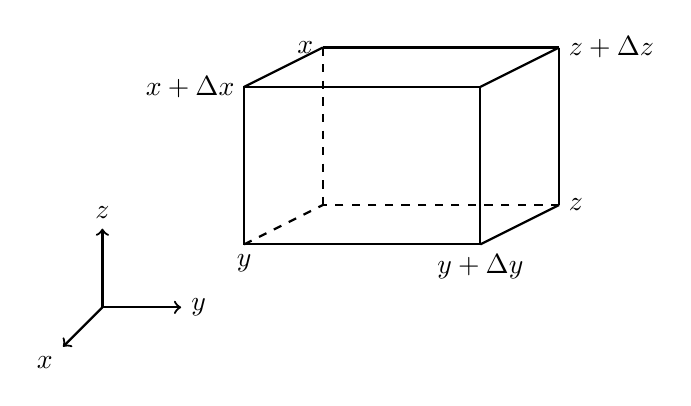
\begin{tikzpicture}
      % 頂点の定義
      \coordinate (A) at (0,0);
      \coordinate (B) at (3,0);
      \coordinate (C) at (3,2);
      \coordinate (D) at (0,2);
      \coordinate (E) at (1,0.5);
      \coordinate (F) at (4,0.5);
      \coordinate (G) at (4,2.5);
      \coordinate (H) at (1,2.5);
  
      % 前面の四角形(実線)
      \draw[thick] (A) -- (B) -- (C) -- (D) -- cycle;
      \draw[thick] (D) -- (H);
      \draw[thick] (C) -- (G);
      \draw[thick] (G) -- (H);
      \draw[thick] (B) -- (F);
      \draw[thick] (F) -- (G);
      \draw[thick, dashed] (H) -- (E);
      \draw[thick, dashed] (A) -- (E);
      \draw[thick, dashed] (F) -- (E);

      \node[left] at (H) {$x$};
      \node[left] at (D) {$x+\Delta x$};
      \node[below] at (A) {$y$};
      \node[below] at (B) {$y+\Delta y$};
      \node[right] at (F) {$z$};
      \node[right] at (G) {$z+\Delta z$};

      \begin{scope}[shift={(-1.8,-0.8)}] % 少し左下に移動
        \draw[thick,->] (0,0) -- (1,0) node[right] {$y$}; % x軸
        \draw[thick,->] (0,0) -- (0,1) node[above] {$z$}; % y軸
        \draw[thick,->] (0,0) -- (-0.5,-0.5) node[below left] {$x$}; % z軸
    \end{scope}
  \end{tikzpicture}
  \end{center}
  \caption{Rectangular prism} \label{fig: 1}
\end{figure}

Using the Gauss divergence theorem,
\begin{align*}
  \int_{\Omega} \nabla \cdot \vec{v} dV 
  &= \int_{\partial \Omega} \vec{v} \cdot \vec{dS}\\
  &= \int_{y}^{y+\Delta y} \int_{z}^{z+\Delta z} \left( v_x (x+\Delta x, y^{\prime}, z^{\prime}) - v_x (x, y^{\prime}, z^{\prime}) \right) dz^{\prime} dy^{\prime}\\
  &+ \int_{z}^{z+\Delta z} \int_{x}^{x+\Delta x} \left( v_y (x^{\prime}, y+\Delta y, z^{\prime}) - v_y (x^{\prime}, y, z^{\prime}) \right) dx^{\prime} dz^{\prime}\\
  &+ \int_{x}^{x+\Delta x} \int_{y}^{y+\Delta y} \left( v_z (x^{\prime}, y^{\prime}, z+\Delta z) - v_z (x^{\prime}, y^{\prime}, z) \right) dy^{\prime} dx^{\prime}\\
  &= \int_{y}^{y+\Delta y} \int_{z}^{z+\Delta z} \int_{x}^{x+\Delta x} \frac{\partial v_x}{\partial x} dx^{\prime} dz^{\prime} dy^{\prime}\\
  &+ \int_{z}^{z+\Delta z} \int_{x}^{x+\Delta x} \int_{y}^{y+\Delta y} \frac{\partial v_y}{\partial y} dy^{\prime} dx^{\prime} dz^{\prime}\\
  &+ \int_{x}^{x+\Delta x} \int_{y}^{y+\Delta y} \int_{z}^{z+\Delta z} \frac{\partial v_z}{\partial z} dz^{\prime} dy^{\prime} dx^{\prime}\\
  &= \int_{x}^{x+\Delta x} \int_{y}^{y+\Delta y} \int_{z}^{z+\Delta z} \left( \frac{\partial v_x}{\partial x} + \frac{\partial v_y}{\partial y} + \frac{\partial v_z}{\partial z} \right) dz^{\prime} dy^{\prime} dx^{\prime}\\
  &= \int_{\Omega} \left( \frac{\partial v_x}{\partial x} + \frac{\partial v_y}{\partial y} + \frac{\partial v_z}{\partial z} \right) dV 
\end{align*}
The above equation has to hold at any region $\Omega$. Therefore,
\begin{equation*}
  \nabla \cdot \vec{v} = \frac{\partial v_x}{\partial x} + \frac{\partial v_y}{\partial y} + \frac{\partial v_z}{\partial z}
\end{equation*}


\bigskip


The $x$ component of the curl of $\vec{v}$ is
\begin{align*}
  &\left( \nabla \cdot \vec{v} \right) \cdot \vec{e_x}
  = \lim_{\Delta y, \Delta z \rightarrow 0} \frac{\displaystyle \oint_C \vec{v} \cdot \vec{dr}}{\Delta y \Delta z} \\
  &= \lim_{\Delta y, \Delta z \rightarrow 0} \frac{1}{\Delta y \Delta z} \left( 
    \int_{y}^{y+\Delta y} v_y(x, y^{\prime}, z)dy^{\prime} +\int_{z}^{z+\Delta z} v_z(x, y+\Delta y, z^{\prime})dz^{\prime}  \right. \\
  &\quad + \left. \int_{y+\Delta y}^{y} v_y(x, y^{\prime}, z+\Delta z)dy^{\prime}+ \int_{z+\Delta z}^{z} v_z(x, y, z^{\prime})dz^{\prime}
  \right)\\
  &= \lim_{\Delta y, \Delta z \rightarrow 0} \frac{\int_{z}^{z+\Delta z} (v_z(x, y+\Delta y, z^{\prime}) - v_z(x, y, z^{\prime})) dz^{\prime} - 
  \int_{y}^{y+\Delta y} (v_y(x, y^{\prime}, z+\Delta z) - v_y(x, y^{\prime}, z)) dy^{\prime}}{\Delta y \Delta z}\\
  &= \frac{\partial v_z}{\partial y} - \frac{\partial v_y}{\partial z}
\end{align*}
Similarly, we can compute the $y$ component and $z$ component, and we can obtain
\begin{equation*}
  \nabla \times \vec{v} = \renewcommand{\arraystretch}{2}
  \begin{pmatrix}
      \displaystyle \frac{\partial v_z}{\partial y} - \frac{\partial v_y}{\partial z} \\
      \displaystyle \frac{\partial v_x}{\partial z} - \frac{\partial v_z}{\partial x} \\
      \displaystyle \frac{\partial v_y}{\partial x} - \frac{\partial v_x}{\partial y}
    \end{pmatrix}
\end{equation*}

\begin{theorem}[Green's Theorem]
  \begin{equation*}
    \oint_C P dx + Q dy = \int_{\Gamma} \left( \frac{\partial P}{\partial y} - \frac{\partial Q}{\partial x} \right) dS
  \end{equation*}
  where $\Gamma \in \mathbb{R}^2$ which is closed by a contour $C$
\end{theorem}
\begin{proof}
  Let $\vec{v}$ be defined as follows.
  \begin{equation*}
    \vec{v} = 
    \begin{pmatrix}
      P \\ Q \\ 0
    \end{pmatrix}
  \end{equation*}
Using the Stokes' theorem,
\begin{align*}
  \oint_{C} \vec{v} \cdot \vec{dr}
  &= \oint_C P dx + Q dy \\
  &= \int_{\Gamma} \left( \nabla \times \vec{v} \right) \cdot \vec{ds} \\
  &= \int_{\Gamma}\renewcommand{\arraystretch}{2}
  \begin{pmatrix}
      \displaystyle -\frac{\partial Q}{\partial z} \\
      \displaystyle \frac{\partial P}{\partial z}  \\
      \displaystyle \frac{\partial P}{\partial y} - \frac{\partial Q}{\partial x}
    \end{pmatrix}
    \cdot
    \begin{pmatrix}
      \displaystyle 0 \\
      \displaystyle 0 \\
      \displaystyle 1
    \end{pmatrix}
    dS \\
    &= \int_{\Gamma} \left( \frac{\partial P}{\partial y} - \frac{\partial Q}{\partial x} \right) dS
\end{align*}
\end{proof}

\end{document}